\subsection{Fine-tuning the MILP formulations}

\begin{warningbox}
  This part is in development
\end{warningbox}

\begin{todobox}
  Describe fine-tuning for:
  \begin{CheckList}{Task}
    \Task{open}{The GC content penalty}
    \Task{open}{The plasmidness}
  \end{CheckList}
\end{todobox}

Because of the fragmentation, for a given attribute, we do not have a strict attribute-equivalence between each contig and its corresponding fragment path in the pan-assembly graph.
Formally, if \(\omega{}\) is an attribute defined either for the contigs and the fragments, \(\forall c \in \Contigs{}\) the statement \(\omega_c = \sum_{i \in \Fragments{}(c)} \omega_i\) does not necessarily hold.
We interpret this issue differentially in the GC content case (\MGC{} problem) and the plasmidness case (\MPS{} problem).
\zcref[S]{sec:pbf_iterbin:decomp:mgc:fine_tuned,sec:pbf_iterbin:decomp:mps:fine_tuned} respectively detail the two issues and propose corrective approaches.

Given a contig \(c \in \Contigs{}\), we say it is active if and only if either for its forward or its reverse the link-arcs defining them in the network are active.

\subsubsection{Correct the GC content score}\label{sec:pbf_iterbin:decomp:mgc:fine_tuned}

The calculation of the GC score for a fragment \(i \in \Fragments{}\) does not rely to the belonging of \(i\) in its contigs \(c \in \Contigs{}(i)\).

\begin{questionbox}
  The plasmidness correction is simpler (see~\Cref{sec:pbf_iterbin:decomp:mps:fine_tuned}) because in we just want to add a bonus.
  Here the question is: if the GC scores of the contigs have to be considered, can we choose one or a subset of contigs from those active to correct the GC content score?
  \begin{itemize}
    \item The contig with the highest absolute GC score difference?
    \item The contig with the highest GC Penalties probability score (bonus)?
    \item The contig with the lowest GC Penalties probability score (penalty)?
  \end{itemize}
  On related issue here is: should we choose only one difference, or a subset?
  The sum of relative GC score differences?

  \begin{todobox}
    Choose one and fix what follows
  \end{todobox}
\end{questionbox}

\begin{fixmebox}
  Because of the new attributes definitions, the corrections introductions and definitions must be adapted.
\end{fixmebox}

\begin{definition}{GC score bonus}{frag_gc_bonus}
  \begin{fixmebox}
    The GC penalty has became a GC prob.\ score: adapt the following definition.
  \end{fixmebox}
  Given a contig \(c \in \Contigs{}\) and a GC content interval \(b \in K\), we define \(\dcgcscore{c}{b}\) as the as a positive GC score bonus for the subcontigs of \(c\):
  \[
    \dcgcscore{c}{b} = \max \Set*{
      0,
      \sum_{\substack{
          i \in \Fragments{}(c) \\ i \text{ a subcontig}
      }}
      \parenth*{
        \frac{|i|}{|c|}\gcscore{c}{b} - \gcscore{i}{b}
      }
    }
  \]
  The bonus for the share depends on which contigs they belong.
  Given a share \(j \in \Fragments{}\) and a GC content interval \(b \in K\), we define \(\dsgcscore{j}{c}{b}\) as the positive difference between the GC penalty from the normalization of the fragment penalty according to the contig and the fragment penalty computed independently of the contigs it belongs:
  \[
    \dsgcscore{j}{c}{b} = \max \Set*{
      0,
      \frac{|j|}{|c|} \gcscore{c}{b} - \gcscore{j}{b}
    }
  \]
  \begin{questionbox}
    A real equivalence between a contig and the sequence of its fragments should imply the \enquote{bonus} to be possibly negative.
    How to argue in favour of a positive bonus rather than a real correction?

    Be aware that if the deltas can be negatives, then we must change the associated constraints
  \end{questionbox}
\end{definition}

\begin{ideabox}
  As for a contig \(c\),
  \[
    \gcscore{c}{b} \leq \dcgcscore{c}{b} + \sum_{\substack{
        j \in \Fragments{}(c) \\
        j \text{ is a share}
    }}\dsgcscore{j}{c}{b}
  \]
  If we don't want to count twice the share participations, we should define:
  \[
    \dcgcscore{c}{b} = \max \Set*{
      0,
      \gcscore{c}{b} - \sum_{i \in \Fragments{}(c)} \gcscore{i}{b}
    }
  \]
  and if a better contig is active, remove the share participation of the worst.

  \begin{questionbox}
    What should we not count twice a share participation, while if it is counted twice, it is because it is used several times (a repeat).

    Perhaps the best thing is just to add a bonus (or correct, negatively too)
  \end{questionbox}
\end{ideabox}

\begin{definition}{\MGC{} fine-tune variables}{mgc:milp:variables:fine_tune}
  \begin{itemize}
    \item \(x_c \in \Set{0, 1} \, \forall c \in \Contigs{}\) denoting whether the contig \(c\) is active or not.
    \item \(\ctggc{c}{b} \in \Set{0, 1} \, \forall (c, b) \in \Contigs{} \times K\) denoting whether the contig \(c\) participates in the solution and the plasmid GC content is in the interval \(b\) or not.
    \item \(\sgcbonus{j}{b} \in \Reals_{\geq 0} \, \forall \text{ share } j \in \Fragments{}, \forall b \in K\) corresponding to the best GC bonus over the GC content penalty for the share \(j\) when several of its contigs are active, given a GC content interval \(b\).
  \end{itemize}
\end{definition}

\begin{definition}{\MGC{} fine-tune constraint}{milp:mcf:constraints:fine_tune}
  A contig \(c \in \Contigs{}\), is active if and only if all the link-arcs defining \(c\) (or its reverse) are active:
  \begin{align}
    |A_\Links{}(c)|x_c & \leq \sum_{a \in A_\Links{}(c)} y_a \\
    |A_\Links{}(\rev{c})|x_c & \leq \sum_{a \in A_\Links{}(\rev{c})} y_a
  \end{align}

  \begin{questionbox}
    Depending on the question (bonus, penalty, relative correction), modelling the \enquote{if and only if} statement may be required.
  \end{questionbox}

  For each contig \(c \in \Contigs{}\), for each GC content interval \(b \in K\), \(\ctggc{c}{b} = 1\) if and only if contig \(c\) is active and the \(b\) is the solution GC content interval:
  \begin{align}
    \ctggc{c}{b} & \leq x_c & \forall (c, b) \in \Contigs{} \times K \\
    \ctggc{c}{b} & \leq GC_b & \forall (c, b) \in \Contigs{} \times K \\
    \ctggc{c}{b} & \geq x_c + GC_b - 1 & \forall (c, b) \in \Contigs{} \times K
  \end{align}

  For each share \(j \in \Fragments{}\), for each GC content interval \(b \in K\), \(\sgcbonus{j}{b}\) is the best correction \(\dsgcscore{j}{c}{b}\) among the active contigs in \(\Contigs(j)\):
  \begin{equation}
    \sgcbonus{j}{b} \leq \sum_{\substack{
        d \in \Contigs(j) \\ \dsgcscore{j}{d}{b} \\ \geq \dsgcscore{j}{c}{b}
    }} \dsgcscore{j}{d}{b} \ctggc{d}{b} \quad
    \begin{array}[t]{@{}l@{}}
      \forall (j, c, b) \in \Fragments{} \times \Contigs{}(j) \times K \\
      j \text{ is a share}
    \end{array}
  \end{equation}

\end{definition}

\begin{definition}{\MGC{} objective function with correction}{pbf_iterbin:decomp:mcf:obj:fine_tune}
  \begin{fixmebox}
    Depending of the question (bonus, penalty, relative correction), the objective function must be adapted.
  \end{fixmebox}
  The objective function aims to maximize the corrected GC score:
  \begin{equation}
    \max ~ GCCorrectedScore
  \end{equation}
  Where
  \begin{align}
    \begin{split}
      GCCorrectedScore = & \sum_{\substack{
          i \in \Fragments{} \\
          b \in K
      }} \gcprob{i}{b} \fraggc{i}{b} \\
      & - \sum_{\substack{
          c \in \Contigs{} \\
          b \in K
      }} \dcgcscore{c}{b}\ctggc{c}{b} \\
      & - \sum_{\substack{
          \text{share } j \in \Fragments{} \\
          b \in K
      }} \sgcbonus{j}{b}
    \end{split}
  \end{align}
\end{definition}

\subsubsection{Positively correct the plasmidness}\label{sec:pbf_iterbin:decomp:mps:fine_tuned}

Especially when \(\omega_c\) is inferior than the sum, if the flow passes through the fragment path corresponding to this contig, we would like to positively correct the sum to obtain \(\omega_c\).

In what follows, we associate new attributes to the fragments corresponding to the possible positive correction we may add to the objective values.
We then adapt the MILP formulations for the corrections.

\begin{refactorbox}
  The idea of correction/bonus is shared between the GC penalties and the plasmidness.
  Restructure to show the common parts and argue in favour of the bonuses.
\end{refactorbox}

\begin{fixmebox}
  Argument order for plasmidness bonus
\end{fixmebox}

Let \(c_1\) and \(c_2\) be two contigs that share a fragment \(j\), where \(\frac{ |j| }{ |c_1| } \rho_{c_1} \geq \frac{ |j| }{ |c_2| } \rho_{c_2}\)
For simplicity, suppose their fragment sets only contain one share, which is \(j\), and \(j\) does not belong to any other contig (i.e. \(\Contigs(j) = \{c_1, c_2\} \)).
Then:
\[
  \sum_{i \in \Fragments{}(c_1) } \rho_{i} = \plm{j} + \sum_{i \in \Fragments{}(c_1), i \neq j} \frac{ |i| }{ |c_1| } \rho_{c_1} \leq \rho_{c_1} = \sum_{i \in \Fragments{}(c_1) } \frac{ |i| }{ |c_1| } \rho_{c_1}
\]

The difference between the two inequality parts equals to:
\[
  \rho_{c_1} - \sum_{i \in \Fragments{}(c_1) } \rho_{i} = \frac{ |j| }{2} \left(\frac{ \rho_{c_1} }{ |c_1| } - \frac{ \rho_{c_2} }{ |c_2| } \right) \geq 0
\]

If the flow passes through all the link-arcs that define \(c_1\) (links in \(A_\Links{}(c_1)\) or links in \(A_\Links{}(\rev{c_1})\) for the reverse of \(c_1\)), the plasmidness is penalized because of the fragmentation of \(c_1\), particularly because of the plasmidness of the share \(j\).
Without the fragmentation of the contig \(c_1\), the plasmidness would have been higher by the difference.

In the following we present a way to solve this issue.

For all share \(j \in \Fragments{}\), we can define a correction constant relative to a contig \(c \in \Contigs(j)\):
\[
  \dplm{c}{j} = \max \Set*{0, \frac{ |i| }{ |c| }\plm{c} - \plm{j}}
\]

If the flow passes through all the link-arcs defining \(c\) (or its reverse), we positively correct the objective value by \(\dplm{c}{j}\).
When the flow passes through several contigs in \(\Contigs(j)\), we only add once this bonus to the objective value, and this bonus is the best of the \(\dplm{c}{j}\) among the \(c \in \Contigs(j)\), represented by the variable \(\rho cor_j\).

\Cref{fig:correct_share_plasmidness} illustrates the values of the share plasmidness correction variables.

\begin{figure}[htb]
  \centering
  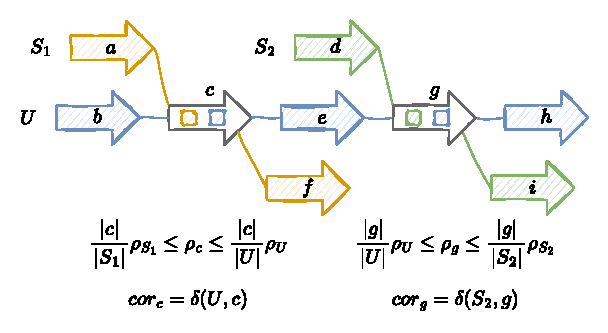
\includegraphics[width=0.6\linewidth]{appendix/ideas/asmcons_milp_fine_tuning/img/constraints-correct_plasmidness_example.pdf}
  \figurecaption{Differential correction of share fragment plasmidness.}{%
    Let assume the flow passes through all the link-arcs defining contigs \(U\), \(S_1\) and \(S_2\) (or their reverse).
    Because of the inequalities between the plasmidness, the objective function is corrected by \(\dplm{U}{c}\) for the share \(c\), and by \(\dplm{S_2}{g}\) for the share \(g\).
  }\label{fig:correct_share_plasmidness}
\end{figure}

\begin{todobox}
  Adapt best bonus GC prob score for plasmidness
\end{todobox}
